%----------------------------------------------------------------------------
\chapter{System Overview}

In this section, the complete system is overviewed. I explain the main design decisions, and some of the more exciting implementation details.

\section{ALPR pipeline}

The applied pipeline aims to compress the traditional tasks into as few steps as possible. The structure is like the one used in WPOD-NET\cite{WPOD-NET}, with some differences.

\begin{figure}[htb]
 \centerline{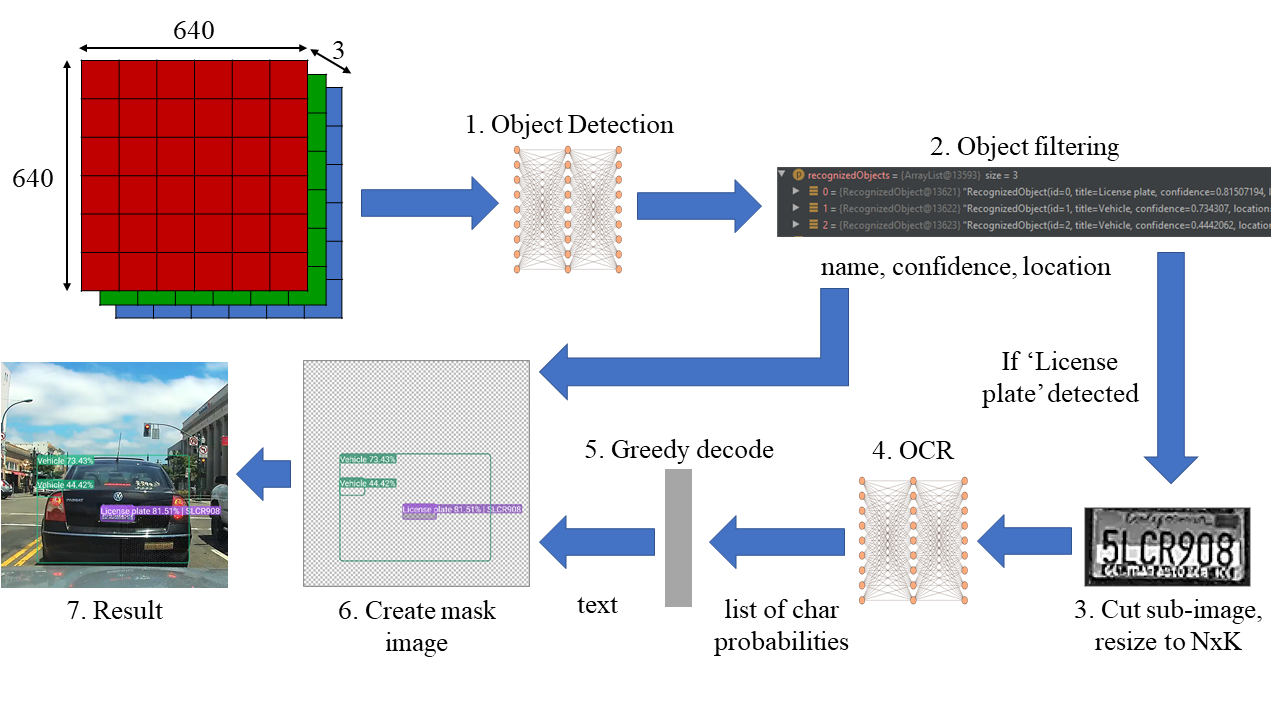
\includegraphics[width=1.0\columnwidth]{.//Figure/System/pipeline.PNG}}
 \caption{The applied ALPR pipeline.}
 \label{fig:simple}
\end{figure}

First, an SSD\cite{SSD} detector is used for both vehicle and plate localization (instead of a YOLO\cite{YOLO9000} vehicle-only detector). The rectification step is excluded from our pipeline, which is a drawback in plate image quality. WPOD-NET's rectification supports only one plate scale, so adding that would not be a general solution, in my opinion. On the other hand, it would increase the computational load as it must run separately for each detected vehicle. The second step is to filter possible plate objects based on location and confidence scores. The third is to cut plate objects from the original image.

The pipeline models are dynamically quantized TensorFlow Lite converted algorithms. On a Samsung Galaxy S10 smartphone, where an image contains only one license plate, the average runtime is roughly 160 ms, including image pre-processing (9 ms), detector inference (75 ms on GPU), plate image part cutting, and resizing (3 ms), OCR inference (37 ms on CPU), Greedy decoding (<1 ms), and creating mask image (33 ms). This runtime may change depending on the number of plates on a picture, as the OCR steps must be repeated on each license plate sub-image.

Besides the best performing model, I also tested the initial architecture (Batch 128). It runs in 37 ms on the device's GPU. Keeping in mind the runtime, it is worth sacrificing marginal quality (+9.5e-3 loss) to acquire a 1.5x speed-up. As a reference, Google's MLKit Vision Text Recognizer\cite{MLKitTextRecognition} ran in 40 ms on the same plate image with a single line of text. The MLKit model is a multiblock recognizer. However, when more than one block is present, its runtime increases drastically.

\begin{table}[htb]
\caption{Running time in milliseconds for OCR models.}
\noindent
\centering
\begin{tabular*}
{\columnwidth}{@{\extracolsep{\stretch{1}}}*{6}{r}@{}}
    & Host & Input & Size [KB] & Loss & Inference [ms]\\ \hline
    $batch 128$ & $CPU$ & $50x500x3$ & $639$ & $0.0848$ & $37$ \\
    $MLKit$ & $CPU$ & $50x500x3$ & $?$ & $?$ & $40$ \\
    $batch 128$ & $GPU$ & $50x500x3$ & $639$ & $0.0848$ & $50$ \\
    $Hyper1st$ & $CPU$ & $50x500x3$ & $4447$ & $0.0753$ & $56$ \\
    $MLKit$ & $CPU$ & $200x200x3$ & $?$ & $?$ & $72$ \\
    $Unfolding$ & $CPU$ & $200x200x3$ & $3133$ & $0.0991$ & $221$ \\
    $Unfolding$ & $GPU$ & $200x200x3$ & $3133$ & $0.0991$ & $372$ \\
\end{tabular*}
\end{table}

\section{Frontend}

The client application’s main task is to detect stolen vehicles, then report them using location and time data. It is possible to run an evaluation on loaded images as well as on the live image feed. The user constantly sees exactly what has been recognized. Stolen vehicle and user data are stored in a local SQLite database, which is synchronized in the background with the API. Camera operations include front/back camera switching, image saving, tap to focus, and pinch to zoom. In the following, I present the Android application’s architecture and the stolen vehicle recognition pipeline.

\subsection{Architecture}

I used the Model View ViewModel (MVVM) UI design pattern. It is an event-driven model, invented by Microsoft to take advantage of data binding capabilities. In MVVM, the View contains UI descriptive code often in a declarative (XML, XAML, HTML) form, and the connection to the ViewModel is realized with explicit data binding. Therefore, there are fewer classic coding tasks in Views, and the business logic components can be easily separated.

There are sub-layers in the model level of the application. I explain their hierarchy through the steps of reporting a single item. Suppose a new stolen vehicle was detected on the live camera feed, and the user selected to report it. In this case, the user sees a ReportActivity, which has a ViewModel storing its UI state. The report item gets stored in a list wrapped in a LiveData object (which is observable from the Activity). When the user clicks on the send button, the related data is transmitted to the RepositoryService in the model layer. Inside this service, there is the ReportRepository. It hides further data operations (database handling, API communication) from the outside. When it receives a new report, it transforms it into a format stored in the Report table and then persists it with ReportDAO (data access object) to the database. After that, it calls ApiService to send the report to the server. When the response arrives from the API, ReportRepository updates the corresponding item in the database. Until the operation is not successful, the user sees the report as pending. Pending items can be deleted or re-sent at any time.

\begin{figure}[htb]
 \centerline{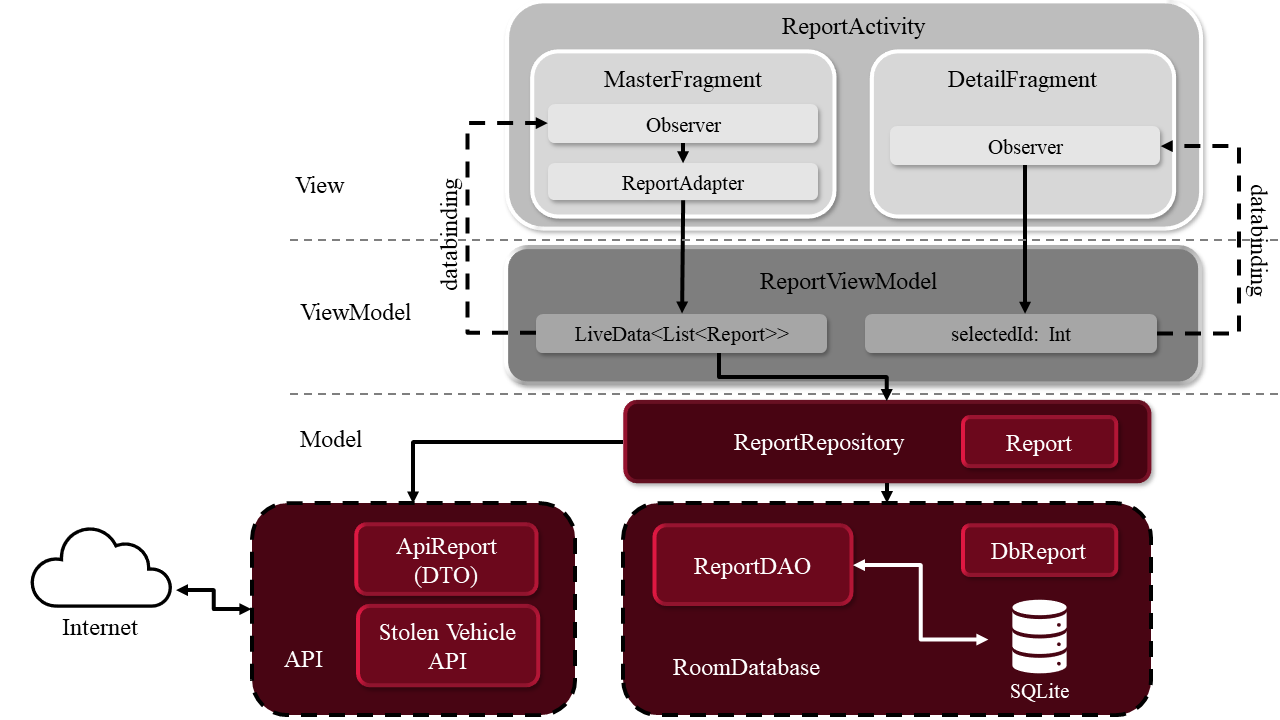
\includegraphics[width=1.0\columnwidth]{.//Figure/System/AndroidArchitecture.png}}
 \caption{MVVM layers in the application.}
 \label{fig:simple}
\end{figure}

\subsection{Database}

Beyond reports, the application stores several other information in its local relational database (list of stolen vehicles, account information, metadata). Outside the relational database, the application stores user preferences as key-value pairs.

\begin{figure}[htb]
 \centerline{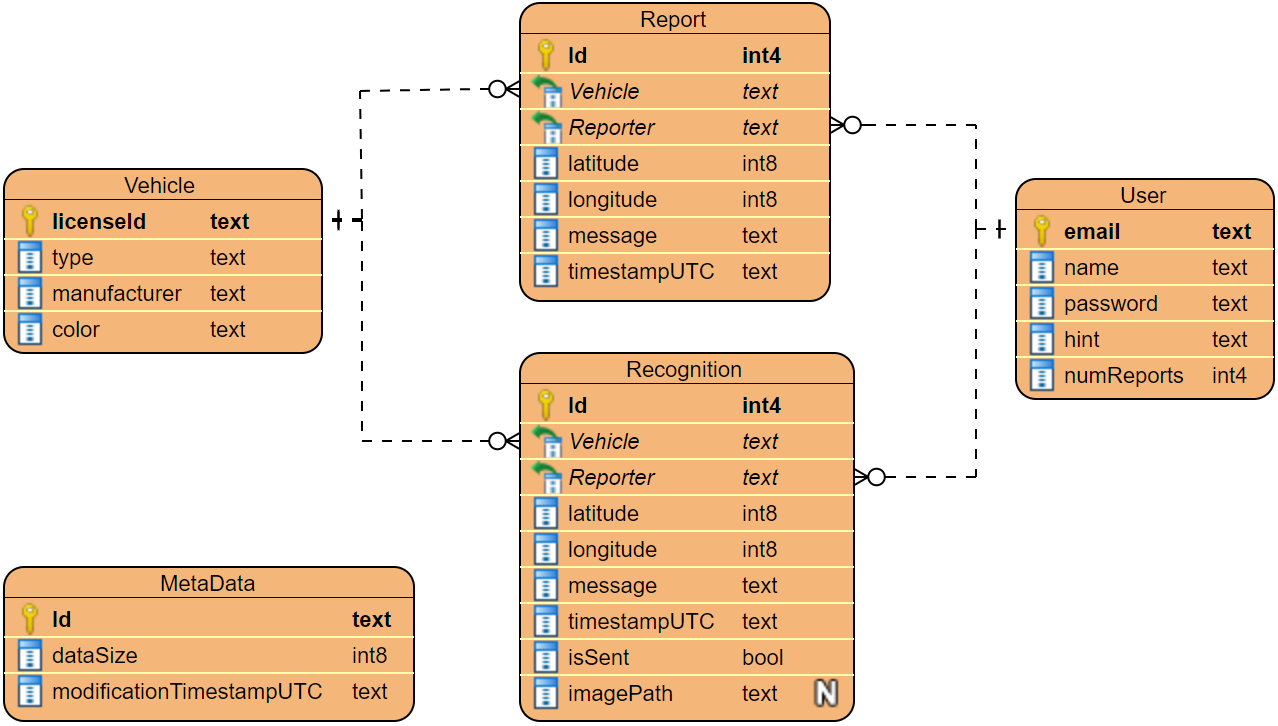
\includegraphics[width=1.0\columnwidth]{.//Figure/System/AppData.PNG}}
 \caption{Application database schema.}
 \label{fig:simple}
\end{figure}

\section{Backend}

The server application provides the API for the clients and manages registered users. It has a stateless REST API, so a user needs to authenticate itself every time querying the server.

\subsection{Architecture}

The server has a three-layered architecture. Because it is responsible for API service and data storage, it does not have a separate View layer (only a simple HTML UI is available).

Instead of the UI layer, there is the communication layer through which the API services can be accessed. It is loosely coupled with other layers. User authentication is done with Http basic authentication.

In the business logic layer, the Authenticator module checks requests and does not allow them to be executed when the required permissions are missing. The Interactor contains the main business logic.

The data access layer contains the DAO classes responsible for handling their tables and providing a unified interface for retrieving/writing data.

\begin{figure}[htb]
 \centerline{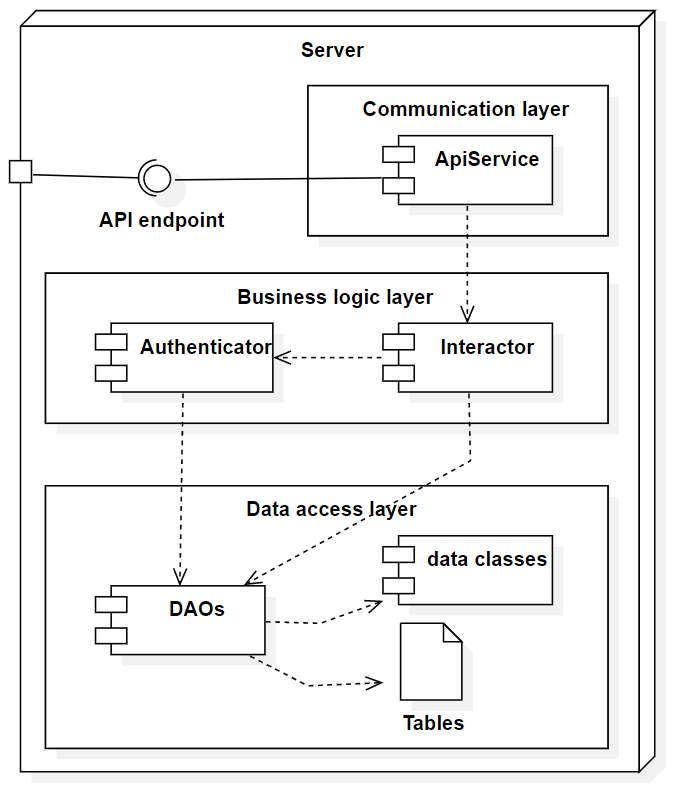
\includegraphics[width=1.0\columnwidth]{.//Figure/System/ServerStructure.PNG}}
 \caption{Structure diagram of the server.}
 \label{fig:simple}
\end{figure}

\subsection{Database}

Since I decided to use a self-created database, I briefly describe its main guidelines. It is a NoSQL variant with an in-memory approach. The tables store information in an object-oriented manner. The table contents are in JSON format (like in the case of MongoDB). To encode/decode JSON files, the server uses the Gson library.

There are tables of stolen vehicles, current reports, and user accounts. To these contents, there are history files(write only) as well. They store all items using a timestamp and a version number to support recovery and traceability. History tables are not stored in memory, and when a data table is updated, its corresponding history is automatically updated. There is a meta content storing size and timestamp information of the previous tables. Lastly, there is an Event table that records system logs (also write-only).

The database serves requests from memory, making API responses fast because there is no need to wait for I/O operations. The memory content is synchronized with the corresponding table in the background. It is a viable solution as a large amount of data is never stored on the server (images are not uploaded). To validate this, I examined one item from the largest JSON object type (Report), which is precisely 173 bytes. Multiplied by 1 million, it turns out that the server needs 173 MB memory, which is acceptable. It is a severe overestimation, though, as the stolen vehicles list obtained by web scraping typically has few thousand items. That is the maximum number of records that the in-memory database ever has (if every stolen vehicle has been detected at once). As history content is only stored persistently, extensive API usage does not saturate the memory either.

\begin{figure}[htb]
 \centerline{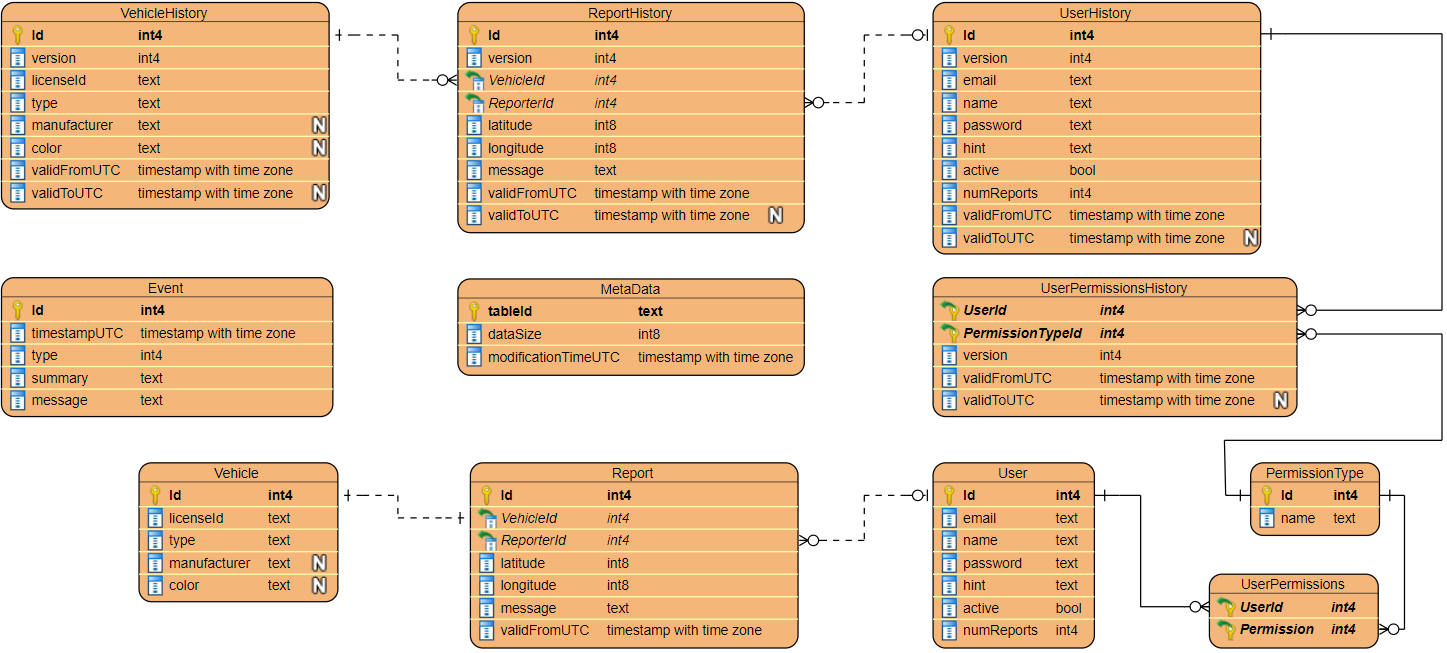
\includegraphics[width=1.0\columnwidth]{.//Figure/System/ServerData.PNG}}
 \caption{Server data schema.}
 \label{fig:simple}
\end{figure}

\subsection{API}

The API is divided into five parts: Vehicles, Reports, Report history, Self, and Users. These names are also the corresponding endpoint prefixes. All parts have similar actions and a unified calling convention. All actions are subject to specific permission, which is evaluated every time before serving. There is also a status page describing the API.

\subsection{Permission}

As the nature of stored data (location and timestamp of stolen vehicles) could potentially allow abuses, there is strict role-based permission model. Users with specific roles are eligible to execute various operations. There are ADMINISTRATOR, API\_REGISTER, SELF\_MODIFY, API\_GET, and API\_SEND permissions.

\begin{itemize}
  \item API\_GET lets an authorized account to download reports.
  \item API\_SEND makes it possible to send recognitions to the server.
  \item SELF\_MODIFY is needed to prevent blacklisted users from deleting themselves and re-register.
  \item An ADMINISTRATOR user can modify the server and any user’s permissions at any time. If someone’s behavior is suspicious, an Admin can revoke permissions, delete a user, or deactivate and blacklist it. An ADMINISTRATOR can register a new user with specific permissions.
  \item The default/guest user in the client application is an account with only an API\_REGISTER role. This way, it is possible for newcomers to register their new accounts. If someone tries to use the application without signing in is, in fact, utilizes this user. As its only API permission is registration, although someone can detect vehicles on-device, he/she cannot report them or see the actual reports. This API\_REGISTER role prevents anyone outside the Android app from registering. The default user can create a new account with SELF\_MODIFY, API\_GET, and API\_SEND permissions.
\end{itemize}
